Soit $f$ une fonction définie et dérivable sur $\R$. On considère les points $A(1;3)$ et $B(3;5)$.

On donne ci-dessous $\mathcal{C}_f$ la courbe représentative de $f$ dans un repère orthogonal du plan, ainsi que la tangente $(AB)$ à la courbe $\mathcal{C}_f$ au point $A$.

\begin{center}
	\begin{tikzpicture}[x=0.8cm,y=0.8cm,xmin=-7,xmax=8,xgrille=1,xgrilles=0.5,ymin=-2,ymax=6,ygrille=1,ygrilles=0.5]
		\GrilleTikz \AxesTikz[ElargirOx=0/0,ElargirOy=0/0]
		\AxexTikz[Police=\footnotesize]{-7,-6,...,7}
		\AxeyTikz[Police=\footnotesize]{-2,-1,...,5}
		\clip (\xmin,\ymin) rectangle (\xmax,\ymax) ;
		\draw[line width=1.25pt,red,domain=\xmin:\xmax,samples=250] plot (\x,{ln(\x*\x+1)+3-ln(2)}) ;
		\draw[red] (-5.5,5.75) node[below,font=\large] {$\mathcal{C}_f$} ;
		\draw[line width=1.25pt,domain=\xmin:\xmax,samples=2,dashed] plot (\x,{\x+2}) ;
		\draw[fill=black] (1,3) circle[radius=1.75pt] node[below right] {$A$} (3,5) circle[radius=1.75pt] node[above left] {$B$} ;
	\end{tikzpicture}
\end{center}

\emph{Les trois parties de l'exercice peuvent être traitées de manière indépendante.}

\bigskip

\textbf{Partie A}

\begin{enumerate}
	\item Déterminer graphiquement les valeurs de $f(1)$ et $f'(1)$.
	\item La fonction $f$ est définie par l'expression $f(x) = \ln \left(ax^2 + 1\right) + b$, où $a$ et $b$ sont des nombres réels positifs.
	\begin{enumerate}
		\item Déterminer l'expression de $f'(x)$.
		\item Déterminer les valeurs de $a$ et $b$ à l'aide des résultats précédents.
	\end{enumerate}
\end{enumerate} 

\textbf{Partie B}

\medskip

On admet que la fonction $f$ est définie sur $\R$ par \[f(x) = \ln \left(x^2 + 1\right) + 3 - \ln (2).\]
%
\begin{enumerate}
	\item Montrer que $f$ est une fonction paire.
	\item Déterminer les limites de $f$ en $+\infty$ et en $-\infty$.
	\item Déterminer l'expression de $f'(x)$.
	
	Étudier le sens de variation de la fonction $f$ sur $\R$.
	
	Dresser le tableau des variations de $f$ en y faisant figurer la valeur exacte du minimum ainsi que les limites de $f$ en $-\infty$ et $+\infty$.
	\item À l'aide du tableau des variations de $f$, donner les valeurs du réel $k$ pour lesquelles l'équation $f(x) = k$ admet deux solutions.
	\item Résoudre l'équation $f(x) = 3 + \ln (2)$.
\end{enumerate}

\textbf{Partie C}

\medskip

On rappelle que la fonction $f$ est définie sur $R$ par $f(x) = \ln \left(x^2 + 1\right) + 3 - \ln (2)$.

\begin{enumerate}
	\item Conjecturer, par lecture graphique, les abscisses des éventuels points d'inflexion de la courbe $\mathcal{C}_f$.
	\item Montrer que, pour tout nombre réel $x$, on a : $f''(x) = \dfrac{2\left(1 - x^2\right)}{\left(x^2 + 1\right)^2}$.
	\item En déduire le plus grand intervalle sur lequel la fonction $f$ est convexe.
\end{enumerate}

\newpage

\section*{ANNEXE à rendre avec la copie}

\begin{center}
	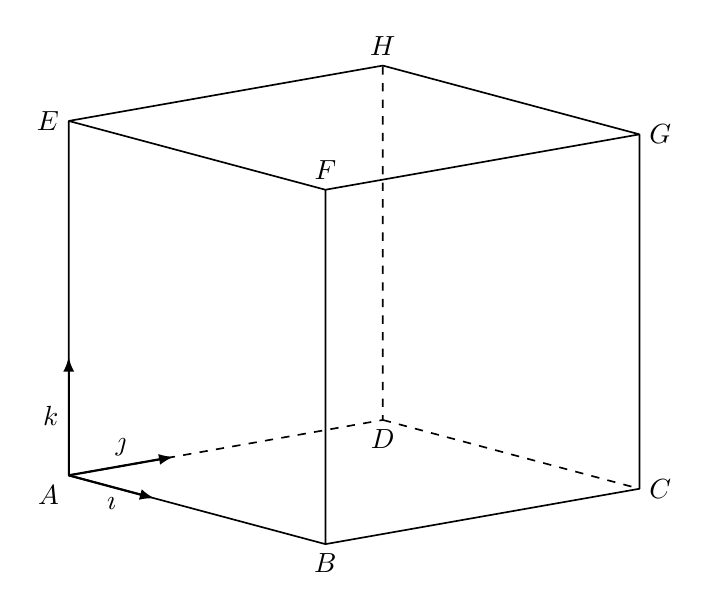
\begin{tikzpicture}[x={(-15:0.75cm)},y={(10:0.9cm)},z={(90:1cm)},line join=bevel,scale=1.5]
		\coordinate (A) at (0,0,0) ; \draw (A) node[below left] {$A$} ;
		\coordinate (B) at (3,0,0) ; \draw (B) node[below] {$B$} ;
		\coordinate (C) at (3,3,0) ; \draw (C) node[right] {$C$} ;
		\coordinate (D) at (0,3,0) ; \draw (D) node[below] {$D$} ;
		\coordinate (E) at (0,0,3) ; \draw (E) node[left] {$E$} ;
		\coordinate (F) at (3,0,3) ; \draw (F) node[above] {$F$} ;
		\coordinate (G) at (3,3,3) ; \draw (G) node[right] {$G$} ;
		\coordinate (H) at (0,3,3) ; \draw (H) node[above] {$H$} ;
		\draw[semithick,dashed] (A)--(D)--(H) (D)--(C) ;
		\draw[semithick] (A)--(B)--(F)--(E)--cycle (B)--(C)--(G)--(F) (G)--(H)--(E) ;
		\draw[thick,->,>=latex] (A)--++(1,0,0) node[midway,below] {$\vect{\imath}$} ;
		\draw[thick,->,>=latex] (A)--++(0,1,0) node[midway,above] {$\vect{\jmath}$} ;
		\draw[thick,->,>=latex] (A)--++(0,0,1) node[midway,left] {$\vect{k}$} ;
	\end{tikzpicture}
\end{center}